\documentclass[a4paper]{book}
\usepackage{a4wide}
\usepackage{makeidx}
\usepackage{graphicx}
\usepackage{multicol}
\usepackage{float}
\usepackage{listings}
\usepackage{color}
\usepackage{textcomp}
\usepackage{alltt}
\usepackage{times}
\usepackage{ifpdf}
\ifpdf
\usepackage[pdftex,
            pagebackref=true,
            colorlinks=true,
            linkcolor=blue,
            unicode
           ]{hyperref}
\else
\usepackage[ps2pdf,
            pagebackref=true,
            colorlinks=true,
            linkcolor=blue,
            unicode
           ]{hyperref}
\usepackage{pspicture}
\fi
\usepackage[utf8]{inputenc}
\usepackage{doxygen}
\lstset{language=C++,inputencoding=utf8,basicstyle=\footnotesize,breaklines=true,breakatwhitespace=true,tabsize=8,numbers=left }
\makeindex
\setcounter{tocdepth}{3}
\renewcommand{\footrulewidth}{0.4pt}
\begin{document}
\hypersetup{pageanchor=false}
\begin{titlepage}
\vspace*{7cm}
\begin{center}
{\Large Procedural Game Plot Generation Prototype }\\
\vspace*{1cm}
{\large Generated by Doxygen 1.6.1}\\
\vspace*{0.5cm}
{\small Fri Jan 22 14:13:34 2010}\\
\end{center}
\end{titlepage}
\clearemptydoublepage
\pagenumbering{roman}
\tableofcontents
\clearemptydoublepage
\pagenumbering{arabic}
\hypersetup{pageanchor=true}
\chapter{Class Index}
\section{Class Hierarchy}
This inheritance list is sorted roughly, but not completely, alphabetically:\begin{DoxyCompactList}
\item \contentsline{section}{Application}{\pageref{classApplication}}{}
\item \contentsline{section}{Decision}{\pageref{classDecision}}{}
\item \contentsline{section}{Decisions}{\pageref{classDecisions}}{}
\item \contentsline{section}{DiscreteRange}{\pageref{classDiscreteRange}}{}
\item \contentsline{section}{GameObject}{\pageref{classGameObject}}{}
\begin{DoxyCompactList}
\item \contentsline{section}{MoveableGameObject}{\pageref{classMoveableGameObject}}{}
\item \contentsline{section}{PlayerCharacter}{\pageref{classPlayerCharacter}}{}
\end{DoxyCompactList}
\item \contentsline{section}{IsometricConversions}{\pageref{classIsometricConversions}}{}
\item \contentsline{section}{Option}{\pageref{classOption}}{}
\item \contentsline{section}{Options}{\pageref{classOptions}}{}
\item \contentsline{section}{Overlay}{\pageref{classOverlay}}{}
\begin{DoxyCompactList}
\item \contentsline{section}{IsometricGrid}{\pageref{classIsometricGrid}}{}
\end{DoxyCompactList}
\item \contentsline{section}{Plot}{\pageref{classPlot}}{}
\item \contentsline{section}{Program}{\pageref{classProgram}}{}
\item \contentsline{section}{RandomGenerator}{\pageref{classRandomGenerator}}{}
\item \contentsline{section}{Result}{\pageref{classResult}}{}
\item \contentsline{section}{World}{\pageref{classWorld}}{}
\end{DoxyCompactList}

\chapter{Class Index}
\section{Class List}
Here are the classes, structs, unions and interfaces with brief descriptions:\begin{DoxyCompactList}
\item\contentsline{section}{\hyperlink{classApplication}{Application} }{\pageref{classApplication}}{}
\item\contentsline{section}{\hyperlink{classDecision}{Decision} }{\pageref{classDecision}}{}
\item\contentsline{section}{\hyperlink{classDecisions}{Decisions} }{\pageref{classDecisions}}{}
\item\contentsline{section}{\hyperlink{classDiscreteRange}{DiscreteRange} }{\pageref{classDiscreteRange}}{}
\item\contentsline{section}{\hyperlink{classGameObject}{GameObject} }{\pageref{classGameObject}}{}
\item\contentsline{section}{\hyperlink{classIsometricConversions}{IsometricConversions} }{\pageref{classIsometricConversions}}{}
\item\contentsline{section}{\hyperlink{classIsometricGrid}{IsometricGrid} }{\pageref{classIsometricGrid}}{}
\item\contentsline{section}{\hyperlink{classMoveableGameObject}{MoveableGameObject} }{\pageref{classMoveableGameObject}}{}
\item\contentsline{section}{\hyperlink{classOption}{Option} }{\pageref{classOption}}{}
\item\contentsline{section}{\hyperlink{classOptions}{Options} }{\pageref{classOptions}}{}
\item\contentsline{section}{\hyperlink{classOverlay}{Overlay} }{\pageref{classOverlay}}{}
\item\contentsline{section}{\hyperlink{classPlayerCharacter}{PlayerCharacter} }{\pageref{classPlayerCharacter}}{}
\item\contentsline{section}{\hyperlink{classPlot}{Plot} }{\pageref{classPlot}}{}
\item\contentsline{section}{\hyperlink{classProgram}{Program} }{\pageref{classProgram}}{}
\item\contentsline{section}{\hyperlink{classRandomGenerator}{RandomGenerator} }{\pageref{classRandomGenerator}}{}
\item\contentsline{section}{\hyperlink{classResult}{Result} }{\pageref{classResult}}{}
\item\contentsline{section}{\hyperlink{classWorld}{World} }{\pageref{classWorld}}{}
\end{DoxyCompactList}

\chapter{Class Documentation}
\hypertarget{classApplication}{
\section{Application Class Reference}
\label{classApplication}\index{Application@{Application}}
}


{\ttfamily \#include $<$Application.h$>$}\subsection*{Public Member Functions}
\begin{DoxyCompactItemize}
\item 
\hypertarget{classApplication_abbda0eddef2dd5fcce957a82373ecb6c}{
virtual int {\bfseries main} (const std::vector$<$ CL\_\-String $>$ \&args)}
\label{classApplication_abbda0eddef2dd5fcce957a82373ecb6c}

\end{DoxyCompactItemize}
\subsection*{Static Public Member Functions}
\begin{DoxyCompactItemize}
\item 
static void \hyperlink{classApplication_a1112e5aede67cff7aad4c8fb4be3e3af}{log} (const int, const CL\_\-String \&)
\end{DoxyCompactItemize}


\subsection{Detailed Description}
The \hyperlink{classApplication}{Application} object provides transition between the modules of the overall application. It instantiates a clanLib window and instantiates the other shared parts of the engine. 

\subsection{Member Function Documentation}
\hypertarget{classApplication_a1112e5aede67cff7aad4c8fb4be3e3af}{
\index{Application@{Application}!log@{log}}
\index{log@{log}!Application@{Application}}
\subsubsection[{log}]{\setlength{\rightskip}{0pt plus 5cm}void Application::log (const int {\em level}, \/  const CL\_\-String \& {\em message})\hspace{0.3cm}{\ttfamily  \mbox{[}static\mbox{]}}}}
\label{classApplication_a1112e5aede67cff7aad4c8fb4be3e3af}
Outputs the message to the console and the active log file. 

The documentation for this class was generated from the following files:\begin{DoxyCompactItemize}
\item 
source/Application.h\item 
source/Application.cpp\end{DoxyCompactItemize}

\hypertarget{classDecision}{
\section{Decision Class Reference}
\label{classDecision}\index{Decision@{Decision}}
}
\subsection*{Public Member Functions}
\begin{DoxyCompactItemize}
\item 
\hypertarget{classDecision_a7b8d8d0b3afb1ac36398d062118f6d6b}{
{\bfseries Decision} (\hyperlink{classPlot}{Plot} $\ast$, const CL\_\-DomElement \&)}
\label{classDecision_a7b8d8d0b3afb1ac36398d062118f6d6b}

\item 
\hypertarget{classDecision_ae6d6d18b9890c8706bd5986978be69b6}{
CL\_\-String {\bfseries getResultAsString} (void)}
\label{classDecision_ae6d6d18b9890c8706bd5986978be69b6}

\item 
\hypertarget{classDecision_a76817bb860641012831b8d5d7857562a}{
int {\bfseries getResultAsInteger} (void)}
\label{classDecision_a76817bb860641012831b8d5d7857562a}

\item 
\hypertarget{classDecision_a8ad5b405e0f154ffe064cb4f548b7931}{
double {\bfseries getResultAsDouble} (void)}
\label{classDecision_a8ad5b405e0f154ffe064cb4f548b7931}

\item 
CL\_\-String \hyperlink{classDecision_a3b4bc70a203e47be88bfdb6d5e059ffb}{getResultType} (void)
\end{DoxyCompactItemize}


\subsection{Member Function Documentation}
\hypertarget{classDecision_a3b4bc70a203e47be88bfdb6d5e059ffb}{
\index{Decision@{Decision}!getResultType@{getResultType}}
\index{getResultType@{getResultType}!Decision@{Decision}}
\subsubsection[{getResultType}]{\setlength{\rightskip}{0pt plus 5cm}CL\_\-String Decision::getResultType (void)}}
\label{classDecision_a3b4bc70a203e47be88bfdb6d5e059ffb}
Returns the type of the value as a string. 

The documentation for this class was generated from the following files:\begin{DoxyCompactItemize}
\item 
source/mystery\_\-xml/Decision.h\item 
source/mystery\_\-xml/Decision.cpp\end{DoxyCompactItemize}

\hypertarget{classDecisions}{
\section{Decisions Class Reference}
\label{classDecisions}\index{Decisions@{Decisions}}
}
\subsection*{Public Member Functions}
\begin{DoxyCompactItemize}
\item 
\hypertarget{classDecisions_a8c89d9f293fd2a70a4c1509a60986382}{
{\bfseries Decisions} (\hyperlink{classPlot}{Plot} $\ast$, const CL\_\-DomElement \&)}
\label{classDecisions_a8c89d9f293fd2a70a4c1509a60986382}

\end{DoxyCompactItemize}


The documentation for this class was generated from the following files:\begin{DoxyCompactItemize}
\item 
source/mystery\_\-xml/\hyperlink{Decisions_8h}{Decisions.h}\item 
source/mystery\_\-xml/\hyperlink{Decisions_8cpp}{Decisions.cpp}\end{DoxyCompactItemize}

\hypertarget{classDiscreteRange}{
\section{DiscreteRange Class Reference}
\label{classDiscreteRange}\index{DiscreteRange@{DiscreteRange}}
}


{\ttfamily \#include $<$DiscreteRange.h$>$}\subsection*{Public Member Functions}
\begin{DoxyCompactItemize}
\item 
\hypertarget{classDiscreteRange_a8191ac666aae46834fce7aa09f11fb11}{
{\bfseries DiscreteRange} (int, int)}
\label{classDiscreteRange_a8191ac666aae46834fce7aa09f11fb11}

\end{DoxyCompactItemize}


\subsection{Detailed Description}
Class for ranges of discrete integers. The constructor defines the start and end integers. Distributions can then be applied to the range of values to influence how they are selected. 

The documentation for this class was generated from the following files:\begin{DoxyCompactItemize}
\item 
mystery\_\-xml/DiscreteRange.h\item 
mystery\_\-xml/DiscreteRange.cpp\end{DoxyCompactItemize}

\hypertarget{classGameObject}{
\section{GameObject Class Reference}
\label{classGameObject}\index{GameObject@{GameObject}}
}
Inheritance diagram for GameObject::\begin{figure}[H]
\begin{center}
\leavevmode
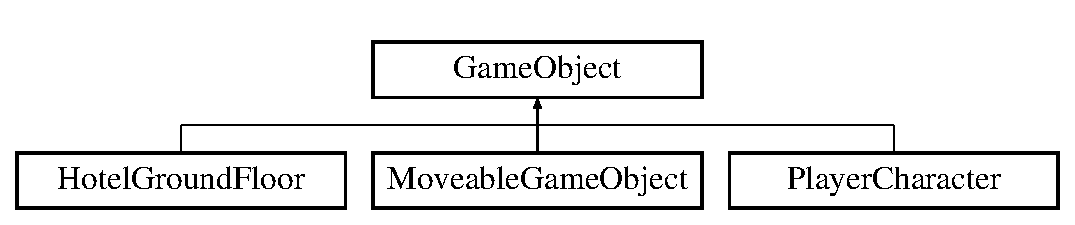
\includegraphics[height=2cm]{classGameObject}
\end{center}
\end{figure}
\subsection*{Public Member Functions}
\begin{DoxyCompactItemize}
\item 
\hyperlink{classGameObject_ad8d1bdb3864097a3723ddac03b947f95}{GameObject} (\hyperlink{classWorld}{World} $\ast$, CL\_\-Pointd \&, CL\_\-Angle \&)
\item 
void \hyperlink{classGameObject_a0eabb72240499a1878b420b5c3f0ecf3}{setDirection} (CL\_\-Angle \&)
\item 
CL\_\-Angle \hyperlink{classGameObject_a456901f9f0b261b206db248960633e50}{getDirection} (void)
\item 
void \hyperlink{classGameObject_a4fd1eeb91d5a220dde7b8574be19b651}{setPosition} (CL\_\-Pointd \&)
\item 
CL\_\-Pointd \hyperlink{classGameObject_adfc89f23ef6d0819c183f1c26bb27e58}{getPosition} (void)
\item 
virtual void \hyperlink{classGameObject_abb64143e72358beb808db22182517802}{draw} ()
\item 
virtual bool \hyperlink{classGameObject_ad2f3cd5d1f5a11b237507cd3ee98b95d}{update} (unsigned int)
\end{DoxyCompactItemize}
\subsection*{Protected Attributes}
\begin{DoxyCompactItemize}
\item 
\hypertarget{classGameObject_adce5bc0f31d7ce307f6bf8fe57030a24}{
\hyperlink{classWorld}{World} $\ast$ {\bfseries world}}
\label{classGameObject_adce5bc0f31d7ce307f6bf8fe57030a24}

\item 
\hypertarget{classGameObject_a9e3a44174a06dd260412d7a13d639d99}{
CL\_\-Pointd {\bfseries position}}
\label{classGameObject_a9e3a44174a06dd260412d7a13d639d99}

\item 
\hypertarget{classGameObject_a8df0dc007367b180dfcd9d2f193f6bdf}{
CL\_\-Angle {\bfseries direction}}
\label{classGameObject_a8df0dc007367b180dfcd9d2f193f6bdf}

\item 
\hypertarget{classGameObject_a5b841978ecf469bc3a69c0d05ad81013}{
CL\_\-Sprite $\ast$ {\bfseries static\_\-sprites} \mbox{[}8\mbox{]}}
\label{classGameObject_a5b841978ecf469bc3a69c0d05ad81013}

\item 
\hypertarget{classGameObject_a22464434abaabf3fb9aab0664dd22eb5}{
CL\_\-Sprite $\ast$ {\bfseries static\_\-current}}
\label{classGameObject_a22464434abaabf3fb9aab0664dd22eb5}

\end{DoxyCompactItemize}


\subsection{Constructor \& Destructor Documentation}
\hypertarget{classGameObject_ad8d1bdb3864097a3723ddac03b947f95}{
\index{GameObject@{GameObject}!GameObject@{GameObject}}
\index{GameObject@{GameObject}!GameObject@{GameObject}}
\subsubsection[{GameObject}]{\setlength{\rightskip}{0pt plus 5cm}GameObject::GameObject ({\bf World} $\ast$ {\em w}, \/  CL\_\-Pointd \& {\em initial\_\-position}, \/  CL\_\-Angle \& {\em initial\_\-direction})}}
\label{classGameObject_ad8d1bdb3864097a3723ddac03b947f95}
param w World$\ast$ param initial\_\-position CL\_\-Pointd The starting position in world coordinates. param initial\_\-direction CL\_\-Angle 

\subsection{Member Function Documentation}
\hypertarget{classGameObject_abb64143e72358beb808db22182517802}{
\index{GameObject@{GameObject}!draw@{draw}}
\index{draw@{draw}!GameObject@{GameObject}}
\subsubsection[{draw}]{\setlength{\rightskip}{0pt plus 5cm}void GameObject::draw (void)\hspace{0.3cm}{\ttfamily  \mbox{[}virtual\mbox{]}}}}
\label{classGameObject_abb64143e72358beb808db22182517802}
Draws the current static sprite for the object. 

Reimplemented in \hyperlink{classMoveableGameObject_a6110e3bcfb088cfaa53bc81ce220bab1}{MoveableGameObject}.\hypertarget{classGameObject_a456901f9f0b261b206db248960633e50}{
\index{GameObject@{GameObject}!getDirection@{getDirection}}
\index{getDirection@{getDirection}!GameObject@{GameObject}}
\subsubsection[{getDirection}]{\setlength{\rightskip}{0pt plus 5cm}CL\_\-Angle GameObject::getDirection (void)}}
\label{classGameObject_a456901f9f0b261b206db248960633e50}
Returns the angle. \hypertarget{classGameObject_adfc89f23ef6d0819c183f1c26bb27e58}{
\index{GameObject@{GameObject}!getPosition@{getPosition}}
\index{getPosition@{getPosition}!GameObject@{GameObject}}
\subsubsection[{getPosition}]{\setlength{\rightskip}{0pt plus 5cm}CL\_\-Pointd GameObject::getPosition (void)}}
\label{classGameObject_adfc89f23ef6d0819c183f1c26bb27e58}
Returns the position in world co-\/ordinates in CL\_\-Pointd. \hypertarget{classGameObject_a0eabb72240499a1878b420b5c3f0ecf3}{
\index{GameObject@{GameObject}!setDirection@{setDirection}}
\index{setDirection@{setDirection}!GameObject@{GameObject}}
\subsubsection[{setDirection}]{\setlength{\rightskip}{0pt plus 5cm}void GameObject::setDirection (CL\_\-Angle \& {\em new\_\-direction})}}
\label{classGameObject_a0eabb72240499a1878b420b5c3f0ecf3}
Sets the direction the game object is facing. This effects the sprite which is used when drawing it. \hypertarget{classGameObject_a4fd1eeb91d5a220dde7b8574be19b651}{
\index{GameObject@{GameObject}!setPosition@{setPosition}}
\index{setPosition@{setPosition}!GameObject@{GameObject}}
\subsubsection[{setPosition}]{\setlength{\rightskip}{0pt plus 5cm}void GameObject::setPosition (CL\_\-Pointd \& {\em new\_\-position})}}
\label{classGameObject_a4fd1eeb91d5a220dde7b8574be19b651}
Sets the position of the object.

param new\_\-position The position as CL\_\-Pointd in terms of world co-\/ordinates. \hypertarget{classGameObject_ad2f3cd5d1f5a11b237507cd3ee98b95d}{
\index{GameObject@{GameObject}!update@{update}}
\index{update@{update}!GameObject@{GameObject}}
\subsubsection[{update}]{\setlength{\rightskip}{0pt plus 5cm}bool GameObject::update (unsigned int {\em time\_\-elapsed\_\-ms})\hspace{0.3cm}{\ttfamily  \mbox{[}virtual\mbox{]}}}}
\label{classGameObject_ad2f3cd5d1f5a11b237507cd3ee98b95d}
Updates any animation in the current sprite. 

Reimplemented in \hyperlink{classMoveableGameObject_af2a5d981743e85b4bd35a90f874b361b}{MoveableGameObject}.

The documentation for this class was generated from the following files:\begin{DoxyCompactItemize}
\item 
source/game/\hyperlink{GameObject_8h}{GameObject.h}\item 
source/game/\hyperlink{GameObject_8cpp}{GameObject.cpp}\end{DoxyCompactItemize}

\hypertarget{classIsometricConversions}{
\section{IsometricConversions Class Reference}
\label{classIsometricConversions}\index{IsometricConversions@{IsometricConversions}}
}
\subsection*{Static Public Member Functions}
\begin{DoxyCompactItemize}
\item 
\hypertarget{classIsometricConversions_a925fb6ecff83501f956092ebd4c237ce}{
static CL\_\-Pointf {\bfseries worldToIsometric} (CL\_\-Pointf)}
\label{classIsometricConversions_a925fb6ecff83501f956092ebd4c237ce}

\item 
\hypertarget{classIsometricConversions_a039c5054ad98fa76218151f39941a3d8}{
static CL\_\-Pointd {\bfseries worldToIsometric} (CL\_\-Pointd)}
\label{classIsometricConversions_a039c5054ad98fa76218151f39941a3d8}

\item 
\hypertarget{classIsometricConversions_a97f4247e5ab8e730432bda5da0be3527}{
static CL\_\-Pointd {\bfseries isometricToWorld} (CL\_\-Pointd)}
\label{classIsometricConversions_a97f4247e5ab8e730432bda5da0be3527}

\end{DoxyCompactItemize}


The documentation for this class was generated from the following files:\begin{DoxyCompactItemize}
\item 
source/game/\hyperlink{IsometricConversions_8h}{IsometricConversions.h}\item 
source/game/\hyperlink{IsometricConversions_8cpp}{IsometricConversions.cpp}\end{DoxyCompactItemize}

\hypertarget{classIsometricGrid}{
\section{IsometricGrid Class Reference}
\label{classIsometricGrid}\index{IsometricGrid@{IsometricGrid}}
}


{\ttfamily \#include $<$IsometricGrid.h$>$}Inheritance diagram for IsometricGrid::\begin{figure}[H]
\begin{center}
\leavevmode
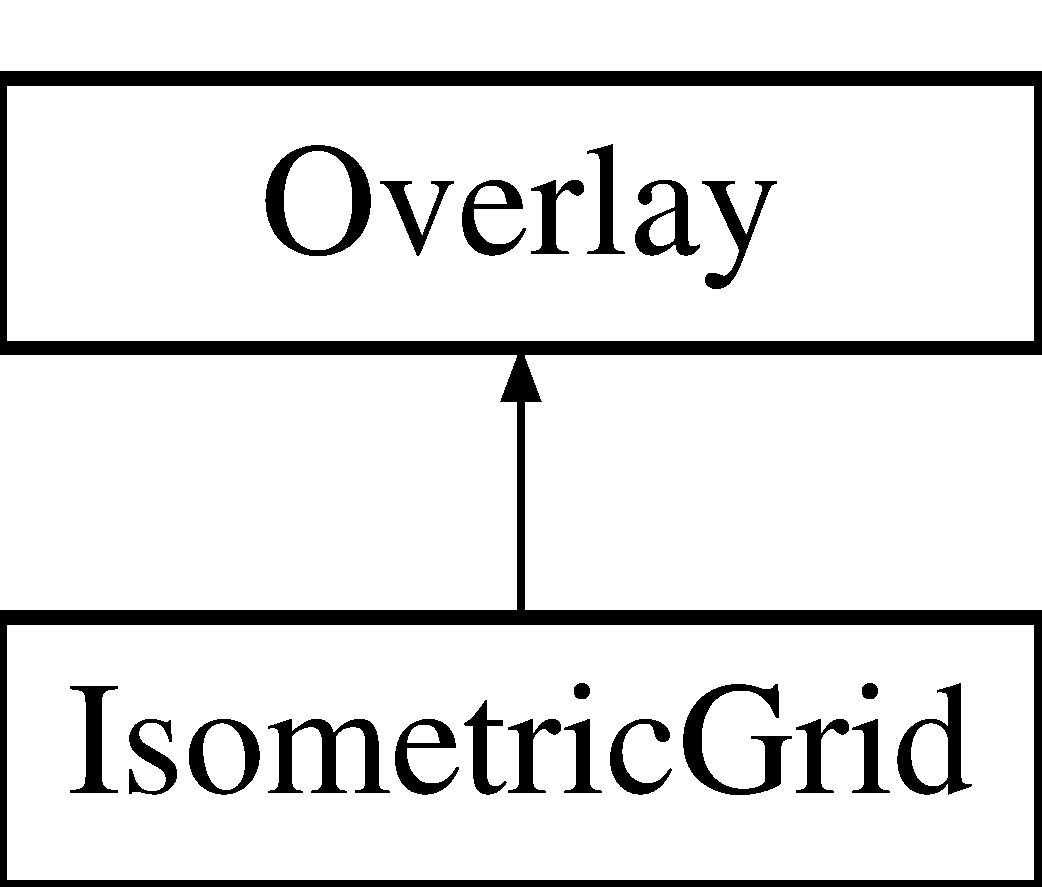
\includegraphics[height=2cm]{classIsometricGrid}
\end{center}
\end{figure}
\subsection*{Public Member Functions}
\begin{DoxyCompactItemize}
\item 
\hypertarget{classIsometricGrid_a4ac39773481a3937b415a71e8e7a29bd}{
{\bfseries IsometricGrid} (\hyperlink{classWorld}{World} $\ast$)}
\label{classIsometricGrid_a4ac39773481a3937b415a71e8e7a29bd}

\item 
\hypertarget{classIsometricGrid_a3138024ea901361f87a47c008fe4f31d}{
void {\bfseries draw} (void)}
\label{classIsometricGrid_a3138024ea901361f87a47c008fe4f31d}

\end{DoxyCompactItemize}


\subsection{Detailed Description}
Constructs a very basic 60x60 isometric grid overlay when calling the draw() function. 

The documentation for this class was generated from the following files:\begin{DoxyCompactItemize}
\item 
IsometricGrid.h\item 
IsometricGrid.cpp\end{DoxyCompactItemize}

\hypertarget{classMoveableGameObject}{
\section{MoveableGameObject Class Reference}
\label{classMoveableGameObject}\index{MoveableGameObject@{MoveableGameObject}}
}
Inheritance diagram for MoveableGameObject::\begin{figure}[H]
\begin{center}
\leavevmode
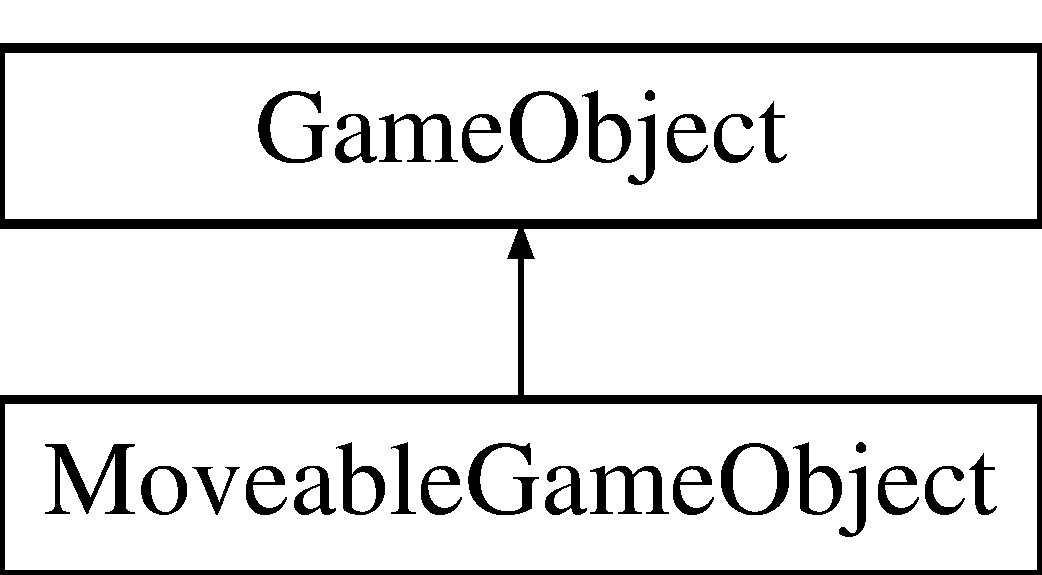
\includegraphics[height=2cm]{classMoveableGameObject}
\end{center}
\end{figure}
\subsection*{Public Member Functions}
\begin{DoxyCompactItemize}
\item 
void \hyperlink{classMoveableGameObject_a6110e3bcfb088cfaa53bc81ce220bab1}{draw} (void)
\item 
bool \hyperlink{classMoveableGameObject_af2a5d981743e85b4bd35a90f874b361b}{update} (unsigned int)
\item 
\hypertarget{classMoveableGameObject_a35e6de5de69921201d48989af9310b71}{
{\bfseries MoveableGameObject} (\hyperlink{classWorld}{World} $\ast$, CL\_\-Pointd \&, CL\_\-Angle \&)}
\label{classMoveableGameObject_a35e6de5de69921201d48989af9310b71}

\end{DoxyCompactItemize}


\subsection{Member Function Documentation}
\hypertarget{classMoveableGameObject_a6110e3bcfb088cfaa53bc81ce220bab1}{
\index{MoveableGameObject@{MoveableGameObject}!draw@{draw}}
\index{draw@{draw}!MoveableGameObject@{MoveableGameObject}}
\subsubsection[{draw}]{\setlength{\rightskip}{0pt plus 5cm}void MoveableGameObject::draw (void)\hspace{0.3cm}{\ttfamily  \mbox{[}virtual\mbox{]}}}}
\label{classMoveableGameObject_a6110e3bcfb088cfaa53bc81ce220bab1}
Draws the current static sprite for the object. 

Reimplemented from \hyperlink{classGameObject_abb64143e72358beb808db22182517802}{GameObject}.\hypertarget{classMoveableGameObject_af2a5d981743e85b4bd35a90f874b361b}{
\index{MoveableGameObject@{MoveableGameObject}!update@{update}}
\index{update@{update}!MoveableGameObject@{MoveableGameObject}}
\subsubsection[{update}]{\setlength{\rightskip}{0pt plus 5cm}bool MoveableGameObject::update (unsigned int {\em time\_\-elapsed\_\-ms})\hspace{0.3cm}{\ttfamily  \mbox{[}virtual\mbox{]}}}}
\label{classMoveableGameObject_af2a5d981743e85b4bd35a90f874b361b}
Updates any animation in the current sprite. 

Reimplemented from \hyperlink{classGameObject_ad2f3cd5d1f5a11b237507cd3ee98b95d}{GameObject}.

The documentation for this class was generated from the following files:\begin{DoxyCompactItemize}
\item 
source/game/\hyperlink{MoveableGameObject_8h}{MoveableGameObject.h}\item 
source/game/\hyperlink{MoveableGameObject_8cpp}{MoveableGameObject.cpp}\end{DoxyCompactItemize}

\hypertarget{classOption}{
\section{Option Class Reference}
\label{classOption}\index{Option@{Option}}
}
\subsection*{Public Member Functions}
\begin{DoxyCompactItemize}
\item 
\hypertarget{classOption_a3cd7af3fd09c247d01e6725e24a91ea2}{
{\bfseries Option} (\hyperlink{classPlot}{Plot} $\ast$, const CL\_\-DomElement \&)}
\label{classOption_a3cd7af3fd09c247d01e6725e24a91ea2}

\item 
\hypertarget{classOption_aa4598f77bf8564c48e3e7b82cd06ed7f}{
int {\bfseries getId} (void)}
\label{classOption_aa4598f77bf8564c48e3e7b82cd06ed7f}

\end{DoxyCompactItemize}


The documentation for this class was generated from the following files:\begin{DoxyCompactItemize}
\item 
mystery\_\-xml/Option.h\item 
mystery\_\-xml/Option.cpp\end{DoxyCompactItemize}

\hypertarget{classOptions}{
\section{Options Class Reference}
\label{classOptions}\index{Options@{Options}}
}
\subsection*{Public Member Functions}
\begin{DoxyCompactItemize}
\item 
\hypertarget{classOptions_a7724e0a467faf1a7538c7345400c0e3f}{
{\bfseries Options} (\hyperlink{classPlot}{Plot} $\ast$, const CL\_\-DomElement \&)}
\label{classOptions_a7724e0a467faf1a7538c7345400c0e3f}

\item 
\hyperlink{classResult}{Result} \hyperlink{classOptions_af944d166a9889b2ff225fe163ab92671}{select} (void)
\end{DoxyCompactItemize}


\subsection{Member Function Documentation}
\hypertarget{classOptions_af944d166a9889b2ff225fe163ab92671}{
\index{Options@{Options}!select@{select}}
\index{select@{select}!Options@{Options}}
\subsubsection[{select}]{\setlength{\rightskip}{0pt plus 5cm}{\bf Result} Options::select (void)}}
\label{classOptions_af944d166a9889b2ff225fe163ab92671}
Picks a value based on weights and parameters. 

The documentation for this class was generated from the following files:\begin{DoxyCompactItemize}
\item 
source/mystery\_\-xml/\hyperlink{Options_8h}{Options.h}\item 
source/mystery\_\-xml/\hyperlink{Options_8cpp}{Options.cpp}\end{DoxyCompactItemize}

\hypertarget{classOverlay}{
\section{Overlay Class Reference}
\label{classOverlay}\index{Overlay@{Overlay}}
}
Inheritance diagram for Overlay:\begin{figure}[H]
\begin{center}
\leavevmode
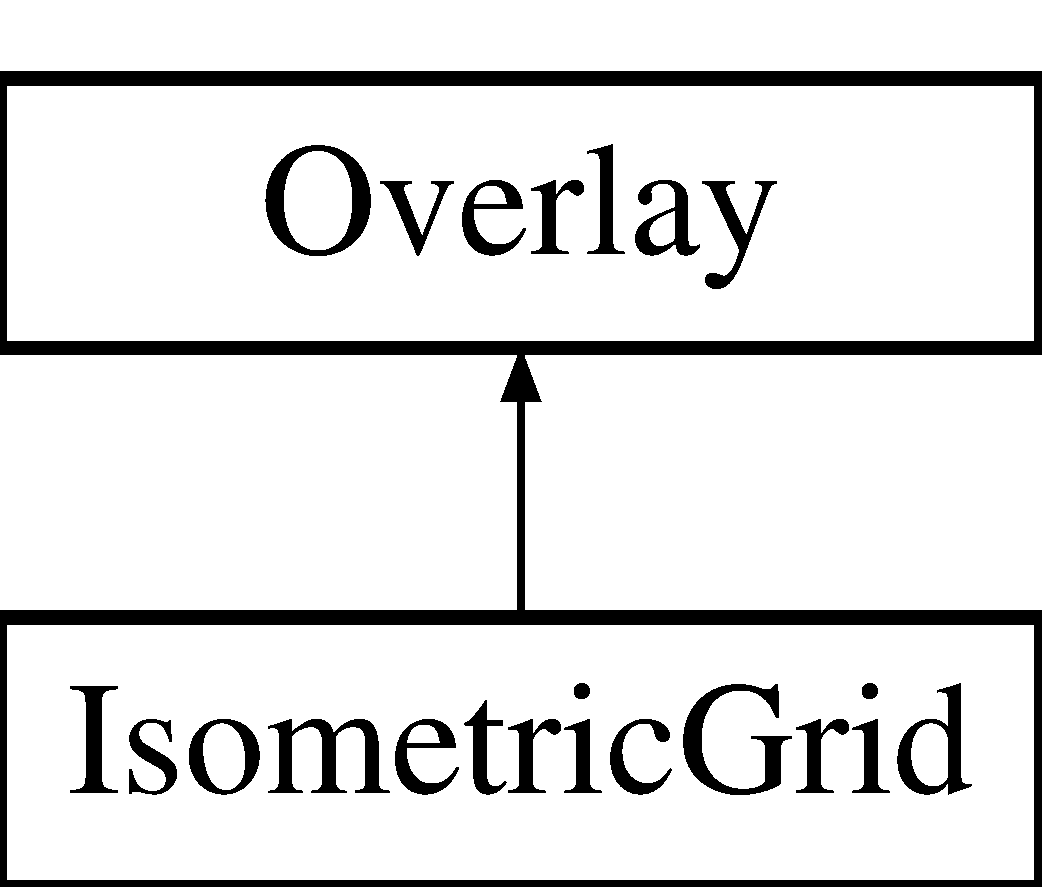
\includegraphics[height=2cm]{classOverlay}
\end{center}
\end{figure}
\subsection*{Public Member Functions}
\begin{DoxyCompactItemize}
\item 
\hypertarget{classOverlay_aecb2ad2cea6041a1b1e332e041daeb13}{
{\bfseries Overlay} (\hyperlink{classWorld}{World} $\ast$)}
\label{classOverlay_aecb2ad2cea6041a1b1e332e041daeb13}

\item 
\hypertarget{classOverlay_a384639128697df8c44c3801ae9212be3}{
virtual void {\bfseries draw} ()=0}
\label{classOverlay_a384639128697df8c44c3801ae9212be3}

\end{DoxyCompactItemize}
\subsection*{Protected Attributes}
\begin{DoxyCompactItemize}
\item 
\hypertarget{classOverlay_aa0de2439856791f770c9e2e9bdc5b613}{
\hyperlink{classWorld}{World} $\ast$ {\bfseries world}}
\label{classOverlay_aa0de2439856791f770c9e2e9bdc5b613}

\end{DoxyCompactItemize}


The documentation for this class was generated from the following files:\begin{DoxyCompactItemize}
\item 
source/game/\hyperlink{Overlay_8h}{Overlay.h}\item 
source/game/\hyperlink{Overlay_8cpp}{Overlay.cpp}\end{DoxyCompactItemize}

\hypertarget{classPlayerCharacter}{
\section{PlayerCharacter Class Reference}
\label{classPlayerCharacter}\index{PlayerCharacter@{PlayerCharacter}}
}
Inheritance diagram for PlayerCharacter::\begin{figure}[H]
\begin{center}
\leavevmode
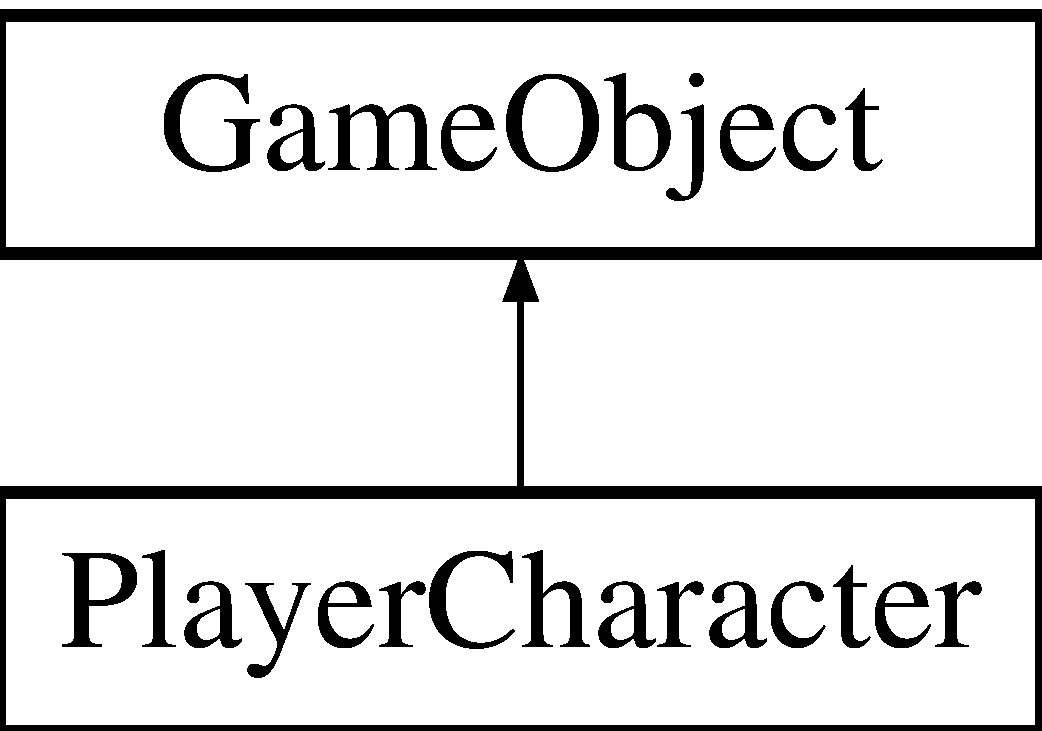
\includegraphics[height=2cm]{classPlayerCharacter}
\end{center}
\end{figure}
\subsection*{Public Member Functions}
\begin{DoxyCompactItemize}
\item 
\hypertarget{classPlayerCharacter_a0207723ef3dc387dcf80b01839715d31}{
{\bfseries PlayerCharacter} (\hyperlink{classWorld}{World} $\ast$, CL\_\-Pointd \&, CL\_\-Angle \&)}
\label{classPlayerCharacter_a0207723ef3dc387dcf80b01839715d31}

\end{DoxyCompactItemize}


The documentation for this class was generated from the following files:\begin{DoxyCompactItemize}
\item 
source/game/\hyperlink{PlayerCharacter_8h}{PlayerCharacter.h}\item 
source/game/\hyperlink{PlayerCharacter_8cpp}{PlayerCharacter.cpp}\end{DoxyCompactItemize}

\hypertarget{classPlot}{
\section{Plot Class Reference}
\label{classPlot}\index{Plot@{Plot}}
}


{\ttfamily \#include $<$Plot.h$>$}\subsection*{Public Member Functions}
\begin{DoxyCompactItemize}
\item 
\hyperlink{classPlot_a836271d0487e811f66768dadb44e4548}{Plot} (const char $\ast$)
\item 
void \hyperlink{classPlot_abdaa02f5857205d8eda001462be0d9f7}{addOption} (\hyperlink{classOption}{Option} $\ast$)
\end{DoxyCompactItemize}


\subsection{Detailed Description}
The plot class is use to parse the plot element in the mystery\_\-xml library. 

\subsection{Constructor \& Destructor Documentation}
\hypertarget{classPlot_a836271d0487e811f66768dadb44e4548}{
\index{Plot@{Plot}!Plot@{Plot}}
\index{Plot@{Plot}!Plot@{Plot}}
\subsubsection[{Plot}]{\setlength{\rightskip}{0pt plus 5cm}Plot::Plot (const char $\ast$ {\em filename})}}
\label{classPlot_a836271d0487e811f66768dadb44e4548}
Constructs a tree from the specified XML file. 

\subsection{Member Function Documentation}
\hypertarget{classPlot_abdaa02f5857205d8eda001462be0d9f7}{
\index{Plot@{Plot}!addOption@{addOption}}
\index{addOption@{addOption}!Plot@{Plot}}
\subsubsection[{addOption}]{\setlength{\rightskip}{0pt plus 5cm}void Plot::addOption ({\bf Option} $\ast$ {\em option})}}
\label{classPlot_abdaa02f5857205d8eda001462be0d9f7}
Adds the \hyperlink{classOption}{Option} object to the map accessible by index. 

The documentation for this class was generated from the following files:\begin{DoxyCompactItemize}
\item 
mystery\_\-xml/Plot.h\item 
mystery\_\-xml/Plot.cpp\end{DoxyCompactItemize}

\hypertarget{classProgram}{
\section{Program Class Reference}
\label{classProgram}\index{Program@{Program}}
}
\subsection*{Static Public Member Functions}
\begin{DoxyCompactItemize}
\item 
\hypertarget{classProgram_a97eed8197e64916a57f1d89477932d7a}{
static int {\bfseries main} (const std::vector$<$ CL\_\-String $>$ \&args)}
\label{classProgram_a97eed8197e64916a57f1d89477932d7a}

\end{DoxyCompactItemize}


The documentation for this class was generated from the following file:\begin{DoxyCompactItemize}
\item 
isometric.cpp\end{DoxyCompactItemize}

\hypertarget{classRandomGenerator}{
\section{RandomGenerator Class Reference}
\label{classRandomGenerator}\index{RandomGenerator@{RandomGenerator}}
}


{\ttfamily \#include $<$RandomGenerator.h$>$}\subsection*{Public Member Functions}
\begin{DoxyCompactItemize}
\item 
\hypertarget{classRandomGenerator_addcda615af9b184d61705dacd0cc0a9a}{
{\bfseries RandomGenerator} (unsigned int)}
\label{classRandomGenerator_addcda615af9b184d61705dacd0cc0a9a}

\item 
\hypertarget{classRandomGenerator_ae10cbb24c2728a4d8d441f2774ac8b99}{
double {\bfseries generateFloat} (void)}
\label{classRandomGenerator_ae10cbb24c2728a4d8d441f2774ac8b99}

\end{DoxyCompactItemize}


\subsection{Detailed Description}
This provides random numbers for the 

The documentation for this class was generated from the following files:\begin{DoxyCompactItemize}
\item 
source/game/\hyperlink{RandomGenerator_8h}{RandomGenerator.h}\item 
source/game/\hyperlink{RandomGenerator_8cpp}{RandomGenerator.cpp}\end{DoxyCompactItemize}

\hypertarget{classResult}{
\section{Result Class Reference}
\label{classResult}\index{Result@{Result}}
}


The documentation for this class was generated from the following files:\begin{DoxyCompactItemize}
\item 
source/mystery\_\-xml/\hyperlink{Result_8h}{Result.h}\item 
source/mystery\_\-xml/\hyperlink{Result_8cpp}{Result.cpp}\end{DoxyCompactItemize}

\hypertarget{classWorld}{
\section{World Class Reference}
\label{classWorld}\index{World@{World}}
}
\subsection*{Public Member Functions}
\begin{DoxyCompactItemize}
\item 
\hyperlink{classWorld_a6ce0c6ba5ce813c0ec0b910a88e09d64}{World} (CL\_\-DisplayWindow \&)
\item 
virtual \hyperlink{classWorld_a8c73fba541a5817fff65147ba47cd827}{$\sim$World} ()
\item 
int \hyperlink{classWorld_a0e3eea96c33cd34c6a3b05bba6b88ef5}{run} ()
\item 
void \hyperlink{classWorld_a6703e4f889e72198e0ede0cd23864792}{addOverlay} (\hyperlink{classOverlay}{Overlay} $\ast$)
\item 
void \hyperlink{classWorld_ad74a2b078f0173249b04e3da2982d081}{addGameObject} (\hyperlink{classGameObject}{GameObject} $\ast$)
\item 
\hypertarget{classWorld_a147bbd276bcff24c6d5c6ade85145545}{
CL\_\-GraphicContext $\ast$ {\bfseries getGC} (void)}
\label{classWorld_a147bbd276bcff24c6d5c6ade85145545}

\item 
\hypertarget{classWorld_ae62ed957ab6a1c8ffd58b5eeda690ce9}{
CL\_\-ResourceManager $\ast$ {\bfseries getRM} (void)}
\label{classWorld_ae62ed957ab6a1c8ffd58b5eeda690ce9}

\end{DoxyCompactItemize}


\subsection{Constructor \& Destructor Documentation}
\hypertarget{classWorld_a6ce0c6ba5ce813c0ec0b910a88e09d64}{
\index{World@{World}!World@{World}}
\index{World@{World}!World@{World}}
\subsubsection[{World}]{\setlength{\rightskip}{0pt plus 5cm}World::World (CL\_\-DisplayWindow \& {\em display\_\-window})}}
\label{classWorld_a6ce0c6ba5ce813c0ec0b910a88e09d64}
Creates the game world and sets up initial contents. \hypertarget{classWorld_a8c73fba541a5817fff65147ba47cd827}{
\index{World@{World}!$\sim$World@{$\sim$World}}
\index{$\sim$World@{$\sim$World}!World@{World}}
\subsubsection[{$\sim$World}]{\setlength{\rightskip}{0pt plus 5cm}World::$\sim$World ()\hspace{0.3cm}{\ttfamily  \mbox{[}virtual\mbox{]}}}}
\label{classWorld_a8c73fba541a5817fff65147ba47cd827}
Destructor. 

\subsection{Member Function Documentation}
\hypertarget{classWorld_ad74a2b078f0173249b04e3da2982d081}{
\index{World@{World}!addGameObject@{addGameObject}}
\index{addGameObject@{addGameObject}!World@{World}}
\subsubsection[{addGameObject}]{\setlength{\rightskip}{0pt plus 5cm}void World::addGameObject ({\bf GameObject} $\ast$ {\em game\_\-object})}}
\label{classWorld_ad74a2b078f0173249b04e3da2982d081}
Adds a game object to the world. \hypertarget{classWorld_a6703e4f889e72198e0ede0cd23864792}{
\index{World@{World}!addOverlay@{addOverlay}}
\index{addOverlay@{addOverlay}!World@{World}}
\subsubsection[{addOverlay}]{\setlength{\rightskip}{0pt plus 5cm}void World::addOverlay ({\bf Overlay} $\ast$ {\em overlay})}}
\label{classWorld_a6703e4f889e72198e0ede0cd23864792}
Adds an overlay object to the world. \hypertarget{classWorld_a0e3eea96c33cd34c6a3b05bba6b88ef5}{
\index{World@{World}!run@{run}}
\index{run@{run}!World@{World}}
\subsubsection[{run}]{\setlength{\rightskip}{0pt plus 5cm}int World::run ()}}
\label{classWorld_a0e3eea96c33cd34c6a3b05bba6b88ef5}
Initiates the game loop. 

The documentation for this class was generated from the following files:\begin{DoxyCompactItemize}
\item 
World.h\item 
World.cpp\end{DoxyCompactItemize}

\printindex
\end{document}
